% !TeX encoding = UTF-8
\documentclass[aspectratio=169]{beamer}
\useoutertheme[progressbar=frametitle]{metropolis}
\useinnertheme{metropolis}
\definecolor{nabgray}{rgb}{0.6,0.59,0.61}
\usecolortheme[named=nabgray]{structure}

\usepackage{tikz}
\usepackage[utf8]{inputenc}
\usepackage[spanish]{babel}
\usepackage{fontspec}
\setmonofont{JetBrains Mono}
\setmainfont{Roboto}
\setsansfont{Roboto}

\usepackage{smartdiagram}
\usepackage{qtree}
\usepackage{verbatim}
\usepackage{svg}
\usepackage{graphicx}
\usepackage{color}

\definecolor{lightgray}{rgb}{0.95, 0.95, 0.95}
\definecolor{darkgray}{rgb}{0.4, 0.4, 0.4}
%\definecolor{purple}{rgb}{0.65, 0.12, 0.82}
\definecolor{editorGray}{rgb}{0.95, 0.95, 0.95}
\definecolor{editorOcher}{rgb}{1, 0.5, 0} % #FF7F00 -> rgb(239, 169, 0)
\definecolor{editorGreen}{rgb}{0, 0.5, 0} % #007C00 -> rgb(0, 124, 0)
\definecolor{orange}{rgb}{1,0.45,0.13}
\definecolor{olive}{rgb}{0.17,0.59,0.20}
\definecolor{brown}{rgb}{0.69,0.31,0.31}
\definecolor{purple}{rgb}{0.38,0.18,0.81}
\definecolor{lightblue}{rgb}{0.1,0.57,0.7}
\definecolor{lightred}{rgb}{1,0.4,0.5}
\usepackage{upquote}
\usepackage{listings}
\lstset{language=java,
	basicstyle=\footnotesize\ttfamily,
	keywordstyle=\footnotesize\color{blue}\ttfamily,
	escapeinside={<@}{@>}
}


\usebackgroundtemplate%
{%
	
\includegraphics[width=\paperwidth]{Images/Contenido}%
}


\title{¿Como funcionan las aplicaciones web}
\author{Víctor Orozco}
\institute{Nabenik}
\date{\today}

\begin{document}





{
    \usebackgroundtemplate{
\includegraphics[width=\paperwidth]{Images/portada}}
    \setbeamercolor{frametitle}{fg=red}
    \usebeamercolor[fg]{normal text}
    \frame{\titlepage}
}


{
	\usebackgroundtemplate{
\includegraphics[width=\paperwidth]{Images/separador}}
	\setbeamercolor{normal text}{fg=white}
	\setbeamercolor{frametitle}{fg=red}
	\usebeamercolor[fg]{normal text}
	\section{Un poco de historia}
}


\begin{frame}{ARPANET}
	\begin{figure}
		\centering
		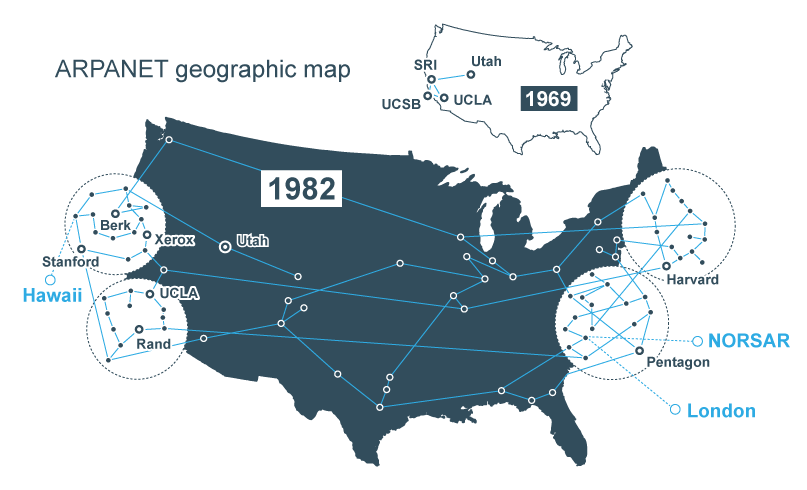
\includegraphics[width=0.7\linewidth]{Images/darpa.png}
	\end{figure}
	
	Problema 1: Una carretera de información (Vinton Cerf y Robert Kahn)
\end{frame}


\begin{frame}{Protocolo}
	\begin{figure}
		\centering
		
\includegraphics[width=0.7\linewidth]{Images/gopher.jpg}
	\end{figure}
\end{frame}



\begin{frame}{Protocolo}
	\begin{figure}
		\centering
		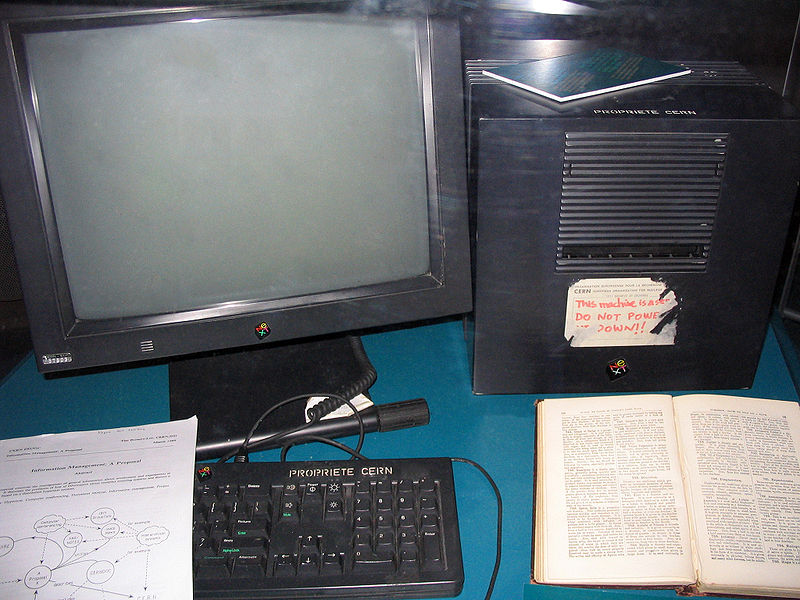
\includegraphics[width=0.5\linewidth]{Images/primer servidor web.jpg}
	\end{figure}
	
	Problema 2: Un lenguaje común (Tim Berners-Lee)
\end{frame}




{
	\usebackgroundtemplate{
\includegraphics[width=\paperwidth]{Images/separador}}
	\setbeamercolor{normal text}{fg=white}
	\setbeamercolor{frametitle}{fg=red}
	\usebeamercolor[fg]{normal text}
	\section{¿Como funcionan las aplicaciones en Internet?}
}


\begin{frame}{Contenido web}
	\begin{figure}
		\centering
		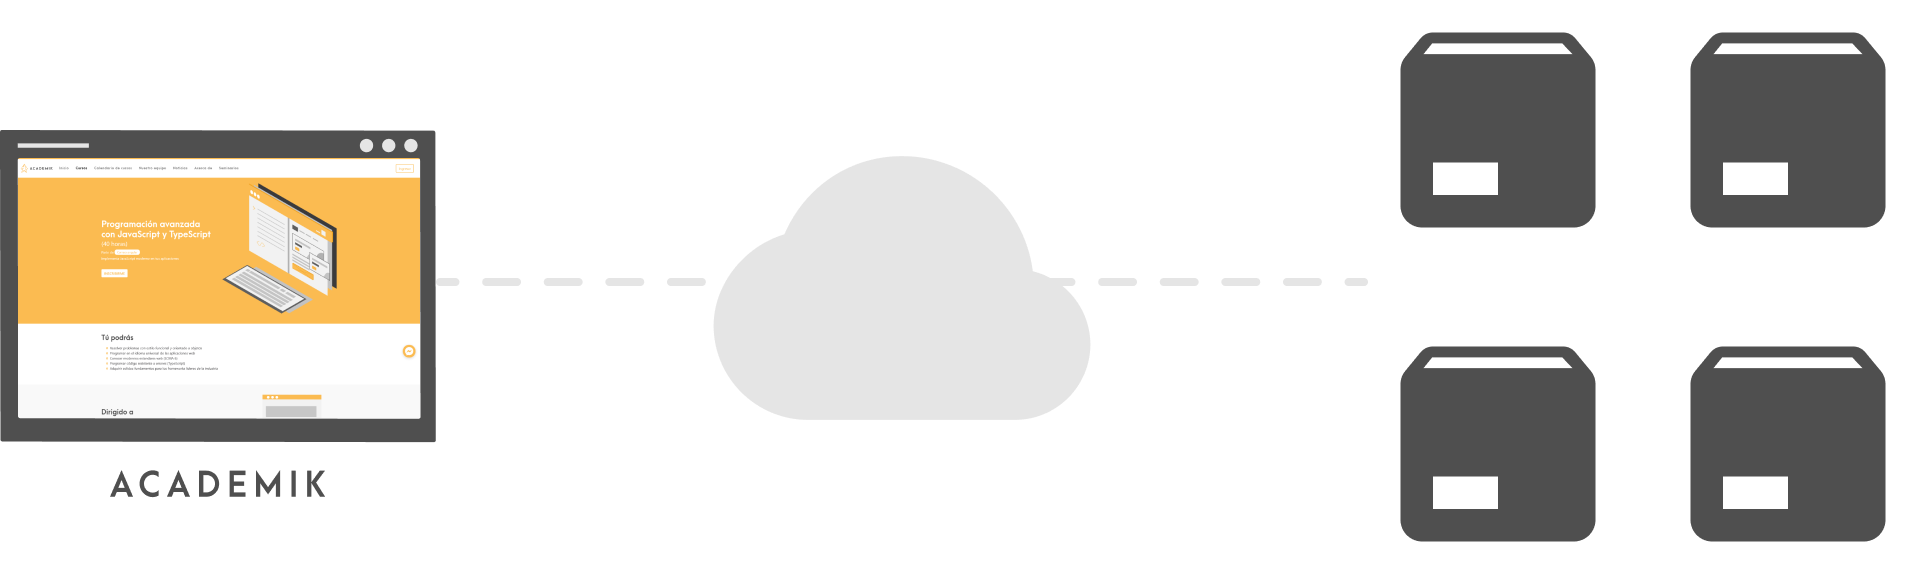
\includegraphics[width=\linewidth]{Images/internet}
	\end{figure}
\end{frame}

\begin{frame}{HTML}
	\begin{figure}
		\centering
		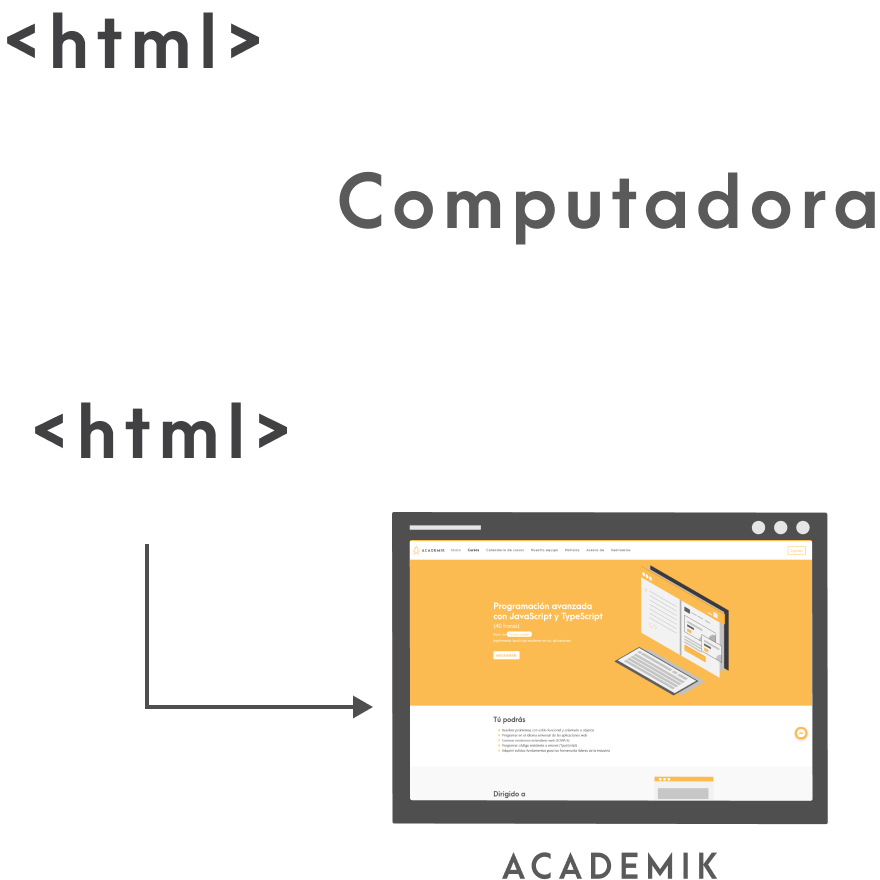
\includegraphics[width=0.50\linewidth]{Images/html.png}
	\end{figure}
\end{frame}


\begin{frame}{Sitio vs aplicación}
	\begin{figure}
		\centering
		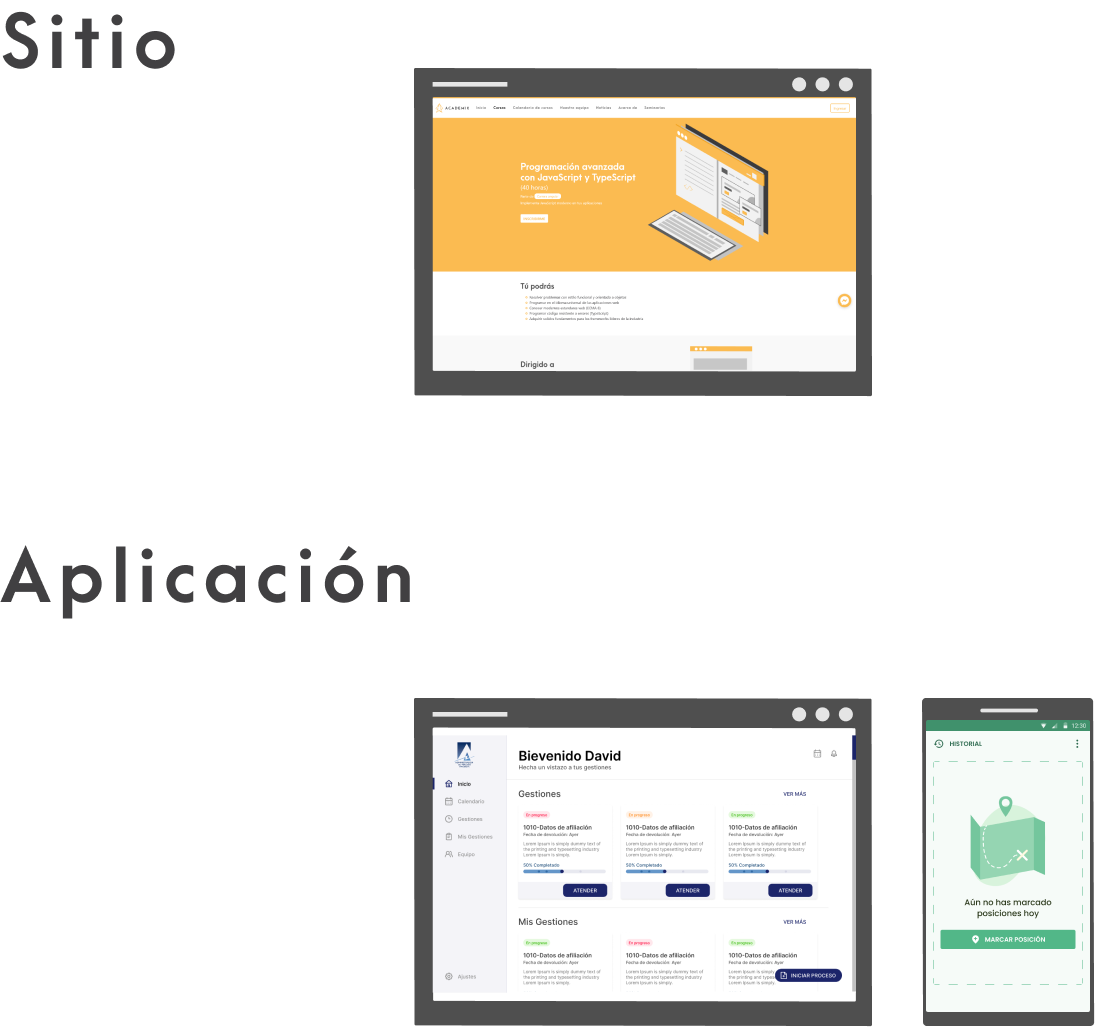
\includegraphics[width=0.55\linewidth]{Images/sitioaplicacion}
	\end{figure}
\end{frame}


{
	\usebackgroundtemplate{
\includegraphics[width=\paperwidth]{Images/separador}}
	\setbeamercolor{normal text}{fg=white}
	\setbeamercolor{frametitle}{fg=red}
	\usebeamercolor[fg]{normal text}
	\section{¿Que habilidades necesito para crear sitios y aplicaciones web?}
}


\begin{frame}{Backend vs frontend}
	\begin{figure}
		\centering
		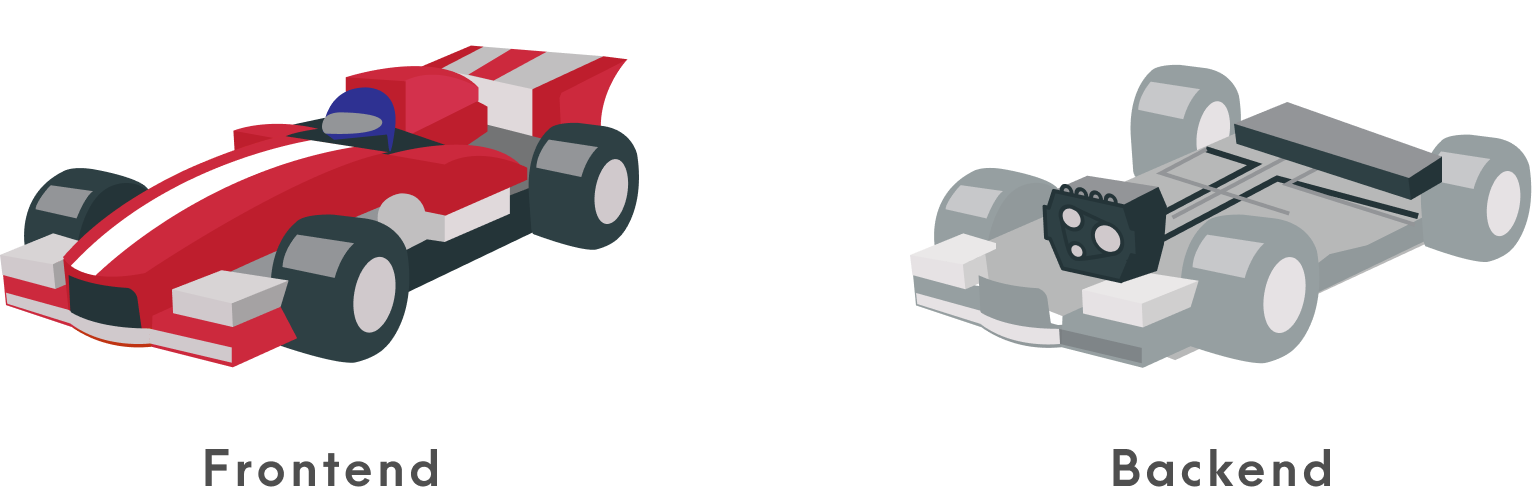
\includegraphics[width=\linewidth]{Images/backvsfront}
	\end{figure}
\end{frame}



\begin{frame}{Backend vs mobile}
	\begin{figure}
		\centering
		
\includegraphics[width=\linewidth]{Images/backvsmobile.png}
	\end{figure}
\end{frame}

\begin{frame}{Habilidades backend}
	\begin{itemize}
		\item Creación de sitios (HTML)
		\item Estilos (CSS, Bootstrap)
		\item Programación (JavaScript, React, Angular)
		\item Administración básica de servidores
		\item Navegadores web
	\end{itemize}
\end{frame}


\begin{frame}{Curso}
	\begin{figure}
		\centering
		
\includegraphics[width=\linewidth]{Images/curso}
	\end{figure}
\end{frame}

\begin{frame}{Horarios}
	\begin{figure}
		\centering
		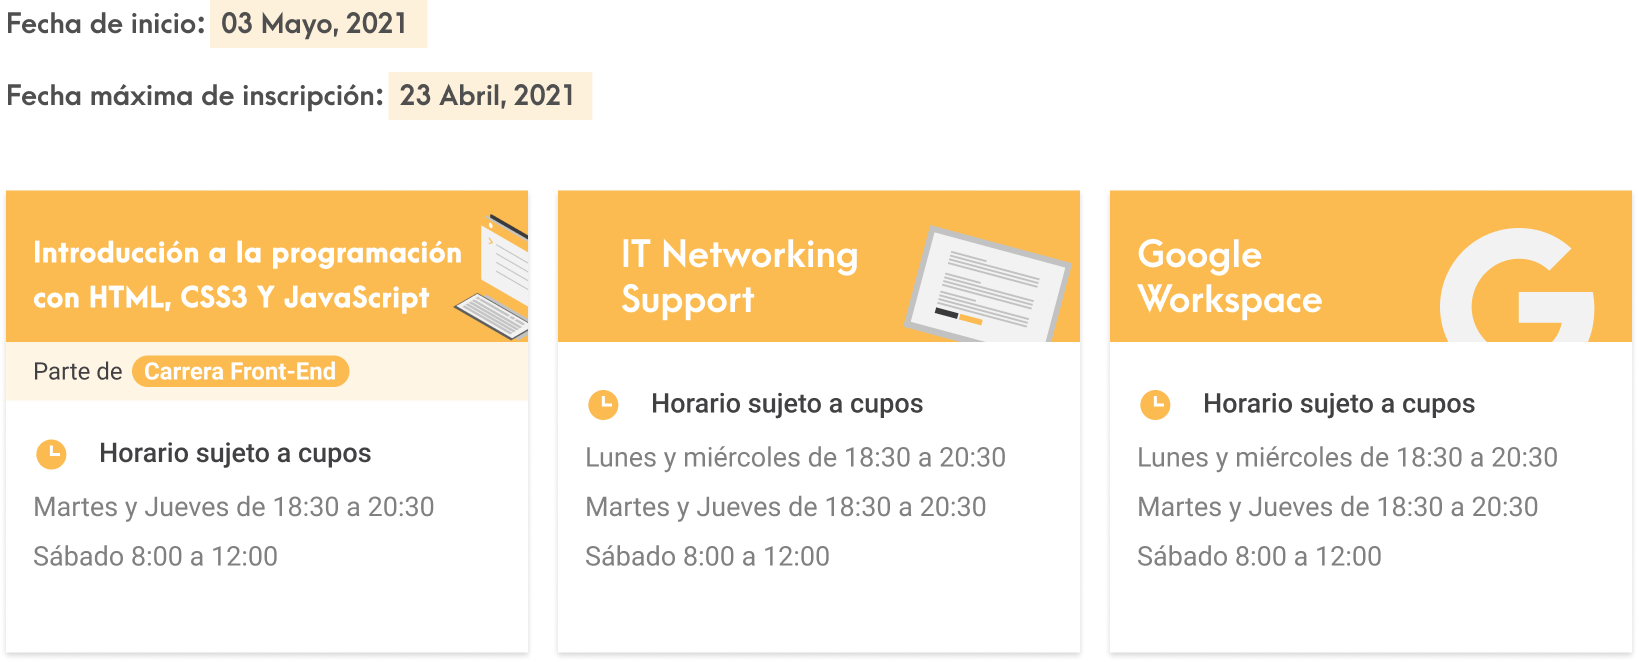
\includegraphics[width=\linewidth]{Images/horarios}
	\end{figure}
\end{frame}



{
	\usebackgroundtemplate{
\includegraphics[width=\paperwidth]{Images/final}}
	\setbeamercolor{normal text}{fg=white}
	\setbeamercolor{frametitle}{fg=red}
	\usebeamercolor[fg]{normal text}
	\section{ }
}



\end{document}
